%!TEX TS-program = xelatex

% Шаблон документа LaTeX создан в 2018 году
% Алексеем Подчезерцевым
% В качестве исходных использованы шаблоны
% 	Данилом Фёдоровых (danil@fedorovykh.ru) 
%		https://www.writelatex.com/coursera/latex/5.2.2
%	LaTeX-шаблон для русской кандидатской диссертации и её автореферата.
%		https://github.com/AndreyAkinshin/Russian-Phd-LaTeX-Dissertation-Template

\documentclass[a4paper,14pt]{article}


%%% Работа с русским языком
\usepackage[english,russian]{babel}   %% загружает пакет многоязыковой вёрстки
\usepackage{fontspec}      %% подготавливает загрузку шрифтов Open Type, True Type и др.
\defaultfontfeatures{Ligatures={TeX},Renderer=Basic}  %% свойства шрифтов по умолчанию
\setmainfont[Ligatures={TeX,Historic}]{Times New Roman} %% задаёт основной шрифт документа
\setsansfont{Comic Sans MS}                    %% задаёт шрифт без засечек
\setmonofont{Courier New}
\usepackage{indentfirst}
\frenchspacing

\renewcommand{\epsilon}{\ensuremath{\varepsilon}}
\renewcommand{\phi}{\ensuremath{\varphi}}
\renewcommand{\kappa}{\ensuremath{\varkappa}}
\renewcommand{\le}{\ensuremath{\leqslant}}
\renewcommand{\leq}{\ensuremath{\leqslant}}
\renewcommand{\ge}{\ensuremath{\geqslant}}
\renewcommand{\geq}{\ensuremath{\geqslant}}
\renewcommand{\emptyset}{\varnothing}

%%% Дополнительная работа с математикой
\usepackage{amsmath,amsfonts,amssymb,amsthm,mathtools} % AMS
\usepackage{icomma} % "Умная" запятая: $0,2$ --- число, $0, 2$ --- перечисление

%% Номера формул
%\mathtoolsset{showonlyrefs=true} % Показывать номера только у тех формул, на которые есть \eqref{} в тексте.
%\usepackage{leqno} % Нумерация формул слева	

%% Перенос знаков в формулах (по Львовскому)
\newcommand*{\hm}[1]{#1\nobreak\discretionary{}
	{\hbox{$\mathsurround=0pt #1$}}{}}

%%% Работа с картинками
\usepackage{graphicx}  % Для вставки рисунков
\graphicspath{{images/}}  % папки с картинками
\setlength\fboxsep{3pt} % Отступ рамки \fbox{} от рисунка
\setlength\fboxrule{1pt} % Толщина линий рамки \fbox{}
\usepackage{wrapfig} % Обтекание рисунков текстом

%%% Работа с таблицами
\usepackage{array,tabularx,tabulary,booktabs} % Дополнительная работа с таблицами
\usepackage{longtable}  % Длинные таблицы
\usepackage{multirow} % Слияние строк в таблице
\usepackage{float}% http://ctan.org/pkg/float

%%% Программирование
\usepackage{etoolbox} % логические операторы


%%% Страница
\usepackage{extsizes} % Возможность сделать 14-й шрифт
\usepackage{geometry} % Простой способ задавать поля
\geometry{top=20mm}
\geometry{bottom=20mm}
\geometry{left=20mm}
\geometry{right=10mm}
%
%\usepackage{fancyhdr} % Колонтитулы
% 	\pagestyle{fancy}
%\renewcommand{\headrulewidth}{0pt}  % Толщина линейки, отчеркивающей верхний колонтитул
% 	\lfoot{Нижний левый}
% 	\rfoot{Нижний правый}
% 	\rhead{Верхний правый}
% 	\chead{Верхний в центре}
% 	\lhead{Верхний левый}
%	\cfoot{Нижний в центре} % По умолчанию здесь номер страницы

\usepackage{setspace} % Интерлиньяж
\onehalfspacing % Интерлиньяж 1.5
%\doublespacing % Интерлиньяж 2
%\singlespacing % Интерлиньяж 1

\usepackage{lastpage} % Узнать, сколько всего страниц в документе.

\usepackage{soul} % Модификаторы начертания

\usepackage{hyperref}
\usepackage[usenames,dvipsnames,svgnames,table,rgb]{xcolor}
\hypersetup{				% Гиперссылки
	unicode=true,           % русские буквы в раздела PDF
	pdftitle={Автоматизация проектных работ},   % Заголовок
	pdfauthor={Солодянкин А.А.},      % Автор
	pdfsubject={Автоматизация проектных работ},      % Тема
	pdfcreator={Солодянкин А.А.}, % Создатель
	pdfproducer={Солодянкин А.А.}, % Производитель
	pdfkeywords={Автоматизация проектных работ}, % Ключевые слова
	colorlinks=true,       	% false: ссылки в рамках; true: цветные ссылки
	linkcolor=black,          % внутренние ссылки
	citecolor=black,        % на библиографию
	filecolor=magenta,      % на файлы
	urlcolor=black           % на URL
}
\makeatletter 
\def\@biblabel#1{#1. } 
\makeatother
\usepackage{cite} % Работа с библиографией
%\usepackage[superscript]{cite} % Ссылки в верхних индексах
%\usepackage[nocompress]{cite} % 
\usepackage{csquotes} % Еще инструменты для ссылок

\usepackage{multicol} % Несколько колонок

\usepackage{tikz} % Работа с графикой
\usepackage{pgfplots}
\usepackage{pgfplotstable}

% ГОСТ заголовки
\usepackage[font=small]{caption}
%\captionsetup[table]{justification=centering, labelsep = newline} % Таблицы по правобу краю
%\captionsetup[figure]{justification=centering} % Картинки по центру


\newcommand{\tablecaption}[1]{\addtocounter{table}{1}\small \begin{flushright}\tablename \ \thetable\end{flushright}%	
\begin{center}#1\end{center}}

\newcommand{\imref}[1]{рис.~\ref{#1}}

\usepackage{multirow}
\usepackage{spreadtab}
\newcolumntype{K}[1]{@{}>{\centering\arraybackslash}p{#1cm}@{}}


\usepackage{xparse}
\usepackage{fancyvrb}

\RecustomVerbatimCommand{\VerbatimInput}{VerbatimInput}
{
	fontsize=\footnotesize    
}

\newcolumntype{?}[1]{!{\vrule width #1}}

\usepackage{tocloft}
\renewcommand{\cftsecleader}{\cftdotfill{\cftdotsep}}
\begin{document} % конец преамбулы, начало документа
\begin{titlepage}
	\begin{center}
		ПРАВИТЕЛЬСТВО РОССИЙСКОЙ ФЕДЕРАЦИИ \\
 		ФЕДЕРАЛЬНОЕ  ГОСУДАРСТВЕННОЕ АВТОНОМНОЕ \\
		ОБРАЗОВАТЕЛЬНОЕ УЧРЕЖДЕНИЕ ВЫСШЕГО ОБРАЗОВАНИЯ\\
		«НАЦИОНАЛЬНЫЙ ИССЛЕДОВАТЕЛЬСКИЙ УНИВЕРСИТЕТ\\
		«ВЫСШАЯ ШКОЛА ЭКОНОМИКИ»
	\end{center}
	
	\begin{center}
		\textbf{Московский институт электроники и математики}
		
		\textbf{Им. А.Н.Тихонова НИУ ВШЭ}
		
		\vspace{2ex}
		
		\textbf{Департамент компьютерной инженерии}
	\end{center}
	\vspace{1ex}	
	
	\vspace{1ex}
	\begin{center}
		\textbf{Практическая работа №7 \\
			<<Математические модели для решения задач размещения на печатной плате>> \\
			по курсу <<Автоматизация проектных работ>>\\
	}
	\end{center}	

	\vspace{2ex}
	\vfill
	
	\vspace{2ex}
	
	\begin{flushright}
		\textbf{Выполнил:}
		
		\vspace{2ex}
		
		Студент группы БИВ174
		
		\vspace{2ex}
		
		Солодянкин Андрей Александрович
		
		\vspace{2ex}
		
		\textbf{Проверил:}
		
		\vspace{2ex}
		
		Новиков Константин Викторович
	\end{flushright}

	\vspace{5ex}
	\begin{center}
		Москва \the\year \, г.
	\end{center}
	
\end{titlepage}
\addtocounter{page}{1}
\tableofcontents
\pagebreak

\section{Задание}

Обеспечить заданную АЧХ транзисторного фильтра таким образом, чтобы частота среза по уровню $0,7*max(K_u)$ = 30 Гц.

\section{Краткие теоретические сведения}

Частотная область удобна при изображении частотного состава сигналов.
Каждая синусоида, представленная на графике, имеет одну частоту. 
Следовательно, в частотной области каждая синусоида представляется только одной частотной составляющей.
Ее амплитуда (на графике - прямая со стрелкой вверх) в частотной области пропорциональна амплитуде синусоиды во временной области. 
Частота f1 соответствует частоте первой синусоиды, а f2 - второй. 
Чем выше частота синусоиды, тем дальше по оси частот она располагается. 
(Словосочетание «частотная составляющая» для краткости заменяют просто на «частоту», если понятно, что речь идет о составляющей частотного спектра, а не о понятии частоты как таковом).

\section{Выполнение работы}

На рис.~\ref{fig:work_1} показаны требуемые АЧХ и схема фильтра.

Были получены следующие параметры фильтра:
$R_1 = 56 kOmh, R_2 = 7 kOmh, R_3 = 6 kOmh, R_4 = 7.45 kOmh, C_1 = 10 uF, C_2 = 8 uF, C_3 = 2.6 uF, C_4 = 8.75 uF$.

На рис.~\ref{fig:work_2} показана демонстрация работы полученных параметров.

\begin{figure}[H]
	\centering
	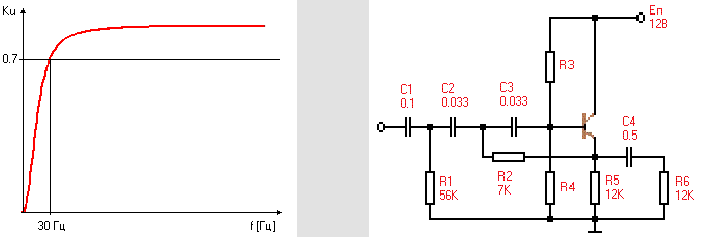
\includegraphics[width=0.9\linewidth]{image/work_1}
	\caption{АЧХ и схема фильтра}
	\label{fig:work_1}
\end{figure}

\begin{figure}[H]
	\centering
	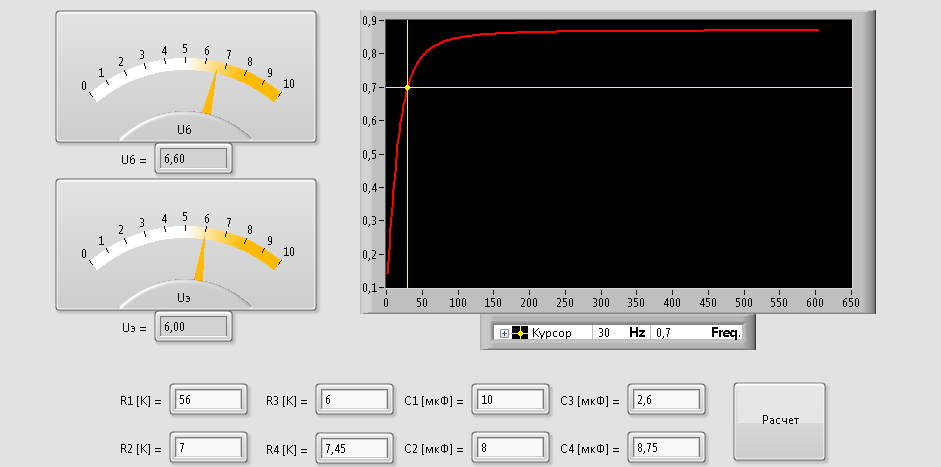
\includegraphics[width=0.9\linewidth]{image/work_2}
	\caption{Полученные параметры фильтра}
	\label{fig:work_2}
\end{figure}

\section{Выводы по работе}

В ходе выполнения лабораторной работы были изучены методы математического моделирования электрических схем в частотной области и способы обеспечения частотных характеристик схем методами математического моделирования.

\section{Контрольные вопросы}

\begin{enumerate}
	\item Математическая модель схемы в частотной области.
	
	В базисе узловых потенциалов математическая модель электрической схемы в частотной области представляет собой систему линейных алгебраических уравнений с комплексными коэффициентами: 
	$$YV=I$$
	где $Y$ -- матрица узловых проводимостей; $V$ -- вектор узловых потенциалов; $I$ -- вектор узловых токов.
	
	Для решения системы линейных уравнений применяют метод $LU$ разложения, в соответствии с которым матрица $Y$ представляется произведением нижней треугольной матрицы с единичной диагональю $L$ и верхней треугольной матрицы $U$:
	$$Y=LU$$
	
	Элементы матриц $L$ и $U$ вычисляются с помощью следующей рекуррентной процедуры:
	
	$$u_{sj} = y_{sj} - \sum_{k=1}^{s-1} l_{sk} u_{kj}, j = s, s+1,..,n;$$
	
	$$l_{is} = \frac{y_{is} - \sum_{k=1}^{s-1} l_{ik} u_{ks}}{u_{ss}}, i = s+1,...,n;$$
	
	После LU разложения матрицы Y, решение системы уравнений заменяется последовательным решением двух систем с треугольными матрицами:
	
	$$ LZ = I; UV=Z$$ 
	
	В результате решения системы уравнений определяется вектор узловых потенциалов, на основе которого рассчитывается комплексный коэффициент передачи, его модуль и фаза:
	
	$$K = \frac{V_j}{V_i}, K = |K| = \sqrt{real^2 K + imag^2 K}, F = arctan \frac{imag K}{real K}$$
	
	\item Методы решения систем линейных алгебраических уравнений.
	
	Есть две группы методов -- прямые и итерационные. 
	
	Прямые методы дают алгоритм, по которому можно найти точное решение систем линейных алгебраических уравнений. Итерационные методы основаны на использовании повторяющегося процесса и позволяют получить решение в результате последовательных приближений.
	
	Некоторые прямые методы:
	
	\begin{itemize}
	\item Метод Гаусса;
	
	\item Метод Крамера;
	
	\item Матричный метод.
	\end{itemize}
	
	Итерационные методы устанавливают процедуру уточнения определённого начального приближения к решению. При выполнении условий сходимости они позволяют достичь любой точности просто повторением итераций. Преимущество этих методов в том, что часто они позволяют достичь решения с заранее заданной точностью быстрее, а также позволяют решать большие системы уравнений. 
	
	
\end{enumerate}

\end{document} % конец документа